\documentclass[../jaynes_prob_theory_notes.tex]{subfiles}
%\usepackage[margin=1in]{geometry}
%\usepackage{amsmath}

\begin{document}

\section{Elementary hypothesis testing}

Reminder: the fundmental principle underlying all probabilistic inference:
\begin{displayquote}
    To form a judgement about the likely truth of falsity of any proposition $A$, the correct procedure is to calculate the probability that $A$ is true, $P(A|E_1E_2\ldots)$, conditional on all the evidence, $E_i$, at hand.
\end{displayquote}

\subsection{Prior probabilities}
\begin{itemize}
    \item When we are given a problem, we have some set of data $D$, but we almost always have some other information $X$, which is all our past experience.
        \begin{itemize}
            \item so all probabilities are conditional, at least in some part, on $X$, so the probability of proposition $A$ is $P(A|DX)$
            \item any probability that is conditional on $X$ alone, $P(A|X)$ is called a \textit{prior probability}
            \item note that \textit{prior} does not necessarily mean ``earlier in time'' it merely denotes information outside the scope of $D$
        \end{itemize}
    \item four general principles for assigning priors:
        \begin{enumerate}
            \item group invariance
            \item maximum entropy
            \item marginalization
            \item coding theory
        \end{enumerate}
    \item in sampling theory, the probabilities that arise presuppose the contents of the population, and seek to predict the data we would get from drawing from that population
        \begin{itemize}
            \item however, most scientific inference requires us to look at problems the other way, alreading knowing the data and needing to know the population
            \item for more on sampling theory, see Feller 1950, 1966 and Kendall \& Stuart 1977
        \end{itemize}
    \item generally in hypothesis testing, with a given data $D$, we want to know which set of hypotheses $\{H_1, H_2,\ldots\}$ is most likely true
        \begin{itemize}
            \item begin with the notation:
                \begin{itemize}
                    \item[] $X =$ prior information
                    \item[] $H =$ some hypothesis to be tested
                    \item[] $D =$ the data
                \end{itemize}
            \item using the product rule we can write the probability as:
                \begin{equation*}
                    P(DH|X) = P(D|HX)P(H|X) = P(H|DX)P(D|X)
                \end{equation*}
            \item $P(H|DX)$ is simply a sampling distribution as seen earlier
            \item since we are looking for probabilities that are not conditional on $H$, but are still conditional on $X$, we need separate notations for them:
                \begin{equation}
                    \label{hyptest}
                    P(H|DX) = P(H|X)\frac{P(D|HX)}{P(D|X)}
                \end{equation}
                \begin{itemize}
                    \item $P(H|DX)$ is called a \textit{posterior probability}, which again means logically later, not temporally later
                    \item $\frac{P(D|HX)}{P(D|X)}$ is called the \textit{likelihood}, $L(H)$
                    \item the likelihood $L(H)$ is not itself a probability for $H$< it is a dimensionless factor which may become a probability when multiplied by a prior probability and a normalization factor
                \end{itemize}
            \item the above equation is an essential principle underlying all scientific inference. IF $P(H|DX)$ is close to 1 or 0, we know that the hypothesis $H$ is likely true or false. If close to 1/2, we know that we need more information
        \end{itemize}
\end{itemize}

\subsection{Testing binary hypotheses with binary data}
\begin{itemize}
    \item the simplest nontrivial case of hypothesis testing is one where we have two hypotheses to test using two data values
    \item adapting eq.~\ref{hyptest} to this, we can also write it as the probability that $H$ is false:
        \begin{equation*}
            P(\bar{H}|DX) = P(\bar{H}|X)\frac{P(D|\bar{H}X)}{P(D|X)}
        \end{equation*}
    \item combining the two equations and getting the ratio, we get
        \begin{equation*}
            \frac{P(H|DX)}{P(\bar{H}|DX)} = \frac{P(H|X)}{P(\bar{H}|X)}\frac{P(D|HX)}{P(D|\bar{H}X)}
        \end{equation*}
    and the $P(D|X)$ term cancels
    \item the ratio of the probability that $H$ is true to the probability that $H$ is false is called the \textit{odds}, $O(H|X)$ on the proposition $H$
        \begin{equation*}
            O(H|DX) = O(H|X)\frac{P(D|HX)}{P(D|\bar{H}X)}
        \end{equation*}
    \item so the postieror odds on $H$ are equal to the prior odds multiplied by the likelihood ratio.\ this is a strictly monotonic function of the probability
    \item convenient to write the odds in terms of logarithms, because then we can add the terms.\ $\log_{10}$ is used due to historical purposes
    \item define a new function, calle the \textit{evidence} for $H$ given $D$ and $X$: $e(H|DX) \equiv 10\log_{10}O(H|DX)$
        \begin{itemize}
            \item still a monotonic function of the probability
            \item base 10 multiplied by 10 puts it in terms of decibels (db)
        \end{itemize}
    \item the evidence for $H$ given $D$ is the prior evidence plus the db provided by taking the log of the likelihood:
        \begin{equation*}
            e(H|DX) = e(H|X) + 10\log_{10}\left[ \frac{P(D|HX)}{P(D|\bar{H}X)} \right]
        \end{equation*}
    \item if $D = D_1D_2\ldots$, the above equation is additive wrt the log of the likelihood.\ if $P(D_j|D_{i}HX) = P(D_j|HX)$, $D_i$ and $D_j$ are called logically \textit{independent}.\ important to note that logical independence does not necessitate causal independence, and visa versa 
    \item if all $D_i$ are logically independent given both $(HX)$ and $(\bar{H}X)$, the evidence becomes
        \begin{equation}
            \label{sum_of_likelihoods}
            e(H|DX) = e(H|X) + 10\log_{10}\sum_{i}\log_{10} \left[ \frac{P(D_i|HX)}{P(D_i|\bar{H}X)} \right]
        \end{equation}
		\begin{figure*}[h!]
			\centering
			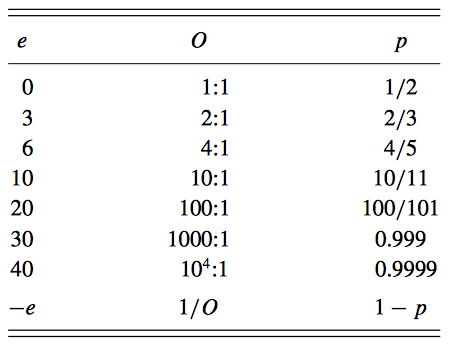
\includegraphics[width=0.3\textwidth]{ev_o_p_table.png}
			\caption{Table comparing the depiction of plausibilities in evidence, odds, and probabilities. Note that evidence provides a better intuitive depiction at $p \rightarrow 0, 1$}
		\end{figure*}
	\item Example: industrial control
	\begin{itemize}
		\item[] $X \equiv$ 11  automatic machines turn out widgets which pour into 11 boxes.\ ten of the machines have a fail rate of one in six.\ the eleventh machine has a fail rate of one in three.\ the output of each machine is collected in an unlabeled box and stored
		\item we choose one of the boxes and test a few of the widgets and classify them as ``good'' or ``bad'' based on the fail rate
		\item Propositions
			\begin{itemize}
				\item[] $A\equiv$ bad batch (1/3 fail)
				\item[] $B\equiv$ good batch (1/6 fail)
			\end{itemize}
		\item prior information $X$ told us there are only two possibilities, therefore $A$ and $B$ are related by negation: $\bar{A} = B$ and $\bar{B} = A$
		\item by the principle of indifference (as we know that there are 11 machines and we do not know which made the batch), we know that $P(A|X) = 1/11$, so
			\begin{equation*}
				e(A|X) = 10\log_{10}\frac{P(A|X)}{P(\bar{A}|X)} = 10\log_{10}\frac{(1/11)}{(10/11)} = -10~\mathrm{db}
			\end{equation*}
			and by necessity, $e(A|X) = +10~\mathrm{db}$
		\item now lets pull out a widget and test for failure.\ if we pull a fail,\ what will that due to the evidence that this is a bad patch?\ Since we know that likelihoods are additive when the log is taken,\ this adds $10\log_{10}\frac{P(\mathrm{bad}|AX)}{P(\mathrm{bad}|\bar{A}X)}$ db to the evidence,\ where $P(\mathrm{result}|AX)$ is the sampling distribution of the result given $A$
			\begin{itemize}
				\item this results in the following probabilities:
					\begin{align*}
						P(\mathrm{bad}|AX) &= \frac{1}{3} & P(\mathrm{good}|AX) &= \frac{2}{3} \\ \\
						P(\mathrm{bad}|BX) &= \frac{1}{6} & P(\mathrm{bad}|BX) &= \frac{5}{6}
					\end{align*}
				\item thus a bad draw will increase the evidence for $A$ by $10\log_{10}\frac{(1/3)}{(1/6)} = 10\log_{10}2 = 3~\mathrm{db}$
				\item pulling a second widget would update the probability according to the hypergeometric distribution (as this is sampling without replacement).\ but if we assume that $N$ is very large,\ we can use the binomial distribution to sample and say that every bad draw will provide +3 db of evidence for hypothesis $A$
				\item a good draw will provide $10\log_{10}\frac{P(\mathrm{good}|AX)}{P(\mathrm{good}|BX)} = 10\log_{10}\frac{(2/3)}{(5/6)} = -0.97~\mathrm{db} \approx -1~\mathrm{db}$ of evidence for hypothesis $A$
				\item so over all, if we draw $n$ widgets, of which $n_b$ are bad and $n_g$ are good, the evidence that the batch is bad is
					\begin{equation*}
						e(A|DX) = e(A|X) + 3n_b - 1n_g
					\end{equation*}
				\item how do we eventually make a decision to reject or accept the batch?
					\begin{itemize}
						\item if we say reject the batch if the evidence for $A$ is $< +0$ db and accept if $> -13$ db,\ this is rejecting or accepting the hypothesis based on the posterior probability
						\item decision making on the posterior probability is called \textit{sequential inference} and denotes that the number of tests is not determined in advance and that the decision is based on the sequence on data values that are found
					\end{itemize}
			\end{itemize}
	\end{itemize}
\end{itemize}

\subsection{Noextensibility beyond the binary case}
    \begin{itemize}
        \item unfortunately, the independent additivity over data (eq.~\ref{sum_of_likelihoods}) and linearity are not general rules 
        \item one could always break up the analysis of a set of hypotheses into a set of binary comparisons to some null hypothesis,\ but this requires $n-1$ calculations
        \item lets examine this reason for nonextensibility in the form of an exercise:
            \begin{itemize}
                \item suppose we have a set of hypotheses $\{H_1, \ldots, H_n\}$ which are mutually exclusive and exhaustive on prior information $X$
                    \begin{equation*}
                        P(H_{i}H_j|X) = P(H_i|X)\delta_{ij} \hspace{1cm} \sum^{n}_{i=1} P(H_i|X) = 1
                    \end{equation*}
                \item we have acquired $m$ data sets $\{D_1, \ldots, D_m\}$, so we can write the probabilities as odds,
                    \begin{equation*}
                        O(H_i|D_1, \ldots, D_{m}X) = O(H_i|X)\frac{P(D_1, \ldots, D_m|H_{i}X)}{P(D_1, \ldots, D_m|\bar{H}_{i}X)}
                    \end{equation*}
                \item commonly, the numerator will factor due to the logical independence of $D_j$ given $H_i$
                    \begin{equation*}
                        P(D_1, \ldots, D_m|H_{i}X) = \prod_{j} P(D_j|H_{i}X), \hspace{0.5cm} 1 \leq i \leq n
                    \end{equation*}
                \item if the denominator can also factor in the same way, into 
                    \begin{equation*}
                        P(D_1, \ldots, D_m|\bar{H}_{i}X) = \prod_{j} P(D_j|\bar{H}_{i}X), \hspace{0.5cm} 1 \leq i \leq n
                    \end{equation*}
                    then the log form of the odds would again become independently additive over $D_j$
                \item however true this is at $n=2$, at $n > 2$, the factorization of the denominator reduces the problem into triviality, because at most one of the factors $\frac{P(D_m|H_{i}X)}{P(D_m|\bar{H}_{i}X)} \neq 1$
            \end{itemize}
    \end{itemize}

\subsection{Multiple hypothesis testing}
    \begin{itemize}
        \item remembering back to the industrial industrial control example, suppose we test 50 widgets and all are fails?\ according to the formula for $e(A|E)$ we would have 150 db of evidence for the proposition of it being a bad batch.
        \item common sense rejects this conclusion, as a bad batch has $1/3$ being failures, not all of them
        \item how do we rectify this and make the testing more ``skeptical'' given an outcome which defies the logic of the original propositions?
        \item let's reconsider the example:
            \begin{itemize}
                \item let's add a proposition $C$ which denotes something going completely wrong with the machine and it gives us a 99\% fail rate
                \item let's give this hypotheses a very low prior probability $P(C|X)$ of $10^{-6}$, or -60 db.
                \item supposing we start out with these initial probabilities
                    \begin{equation*}
                        P(A|X) = \frac{1}{11}(1-10^{-6}) \hspace{0.5cm} P(B|X) = \frac{10}{11}(1-10^{-6}) \hspace{0.5cm} P(C|X) = 10^{-6}
                    \end{equation*}
                where $A$ is a box with $1/3$ defective, $B$ is a box with $1/6$ defective, and $C$ is a box with $99/100$ defective
                \item with $(1-10^{-6})$ being negligible, we start with the initial evidence values $A=-10$ db, $B=+10$ db, and $C=-60$ db
                \item with the data proposition $D$ denoting that $m$ widgets were drawn and were all fails, tehe posterior evidence for proposition $C$ is 
                    \begin{equation*}
                        e(C|DX) = e(C|X) + 10\log_{10} \frac{P(D|CX)}{P(D|\bar{C}X)}
                    \end{equation*}
                \item if $N \gg m$, $P(D|CX) = {\left( \frac{99}{100} \right)}^m$ is the probability that the first $m$ drawn are all bad, if $C$ is true
                \item we also need to know the probability $P(D|\bar{C}X)$:
                    \begin{itemize}
                        \item since there are only three possibilities, $A$, $B$, and $C$, $\bar{C} \Rightarrow A+B$,
                            \begin{equation*}
                                P(\bar{C}|DX) = P(A+B|DX) = P(A|DX) + P(B|DX)
                            \end{equation*}
                        \item we also know that
                            \begin{equation*}
                                P(D|\bar{C}X) = P(D|X)\frac{P(\bar{C}|DX)}{P(\bar{C}|X)}
                            \end{equation*}
                        \item combining these two equations we get
                            \begin{equation*}
                            P(D|\bar{C}X) = \frac{P(D|AX)P(A|X) + P(D|BX)P(B|X)}{P(A|X) + P(B|X)} = {\left( \frac{1}{3} \right)}^m {\left( \frac{1}{11} \right)} + {\left( \frac{1}{6} \right)}^m \frac{10}{11}
                            \end{equation*}
                    \end{itemize}
                \item putting everything together, we have the evidence for proposition $C$,
                    \begin{equation*}
                        e(C|DX) = -60 + 10\log_{10} \left[ \frac{{\left( \frac{99}{100} \right)}^m}{\frac{1}{11} {\left( \frac{1}{3} \right)}^m + \frac{10}{11} {\left( \frac{1}{6} \right)}^m} \right]
                    \end{equation*}
                \item if $m > 5$ is a good approximation, $e(C|DX) \approx -49.6 + 4.73m$ and if $m < 3$ a cruder approximation is $e(C|DX) \approx -60 + 7.73m$
                \item so 10 consecutive bad widgets would raise the evidence for $C$ by $\sim 58$ db, while 11 would make us consider it more likely true than false
                \item what is happening to $A$ and $B$ during this?\ the equations below denote the evidence for the two propositions and their approximate forms
                    \begin{equation*}
                        e(A|DX) = -10 + 10\log_{10} \left[ \frac{{\left( \frac{1}{3} \right)}^m}{{\left( \frac{1}{6} \right)}^m + \frac{11}{10} \times 10^{-6} {\left( \frac{99}{100} \right)}^m} \right] \approx \left[ \begin{matrix} -10+3m & \mathrm{for}~m<7 \\ +49.6-4.73m & \mathrm{for}~m>8 \end{matrix} \right]
                    \end{equation*}
                    \begin{equation*}
                        e(B|DX) = +10 + 10\log_{10} \left[ \frac{{\left( \frac{1}{6} \right)}^m}{{\left( \frac{1}{3} \right)}^m + \frac{11}{10} \times 10^{-6} {\left( \frac{99}{100} \right)}^m} \right] \approx \left[ \begin{matrix} 10-3m & \mathrm{for}~m<10 \\ +59.6-7.73m & \mathrm{for}~m>11 \end{matrix} \right]
                    \end{equation*}
                    \begin{figure}
                        \centering
                        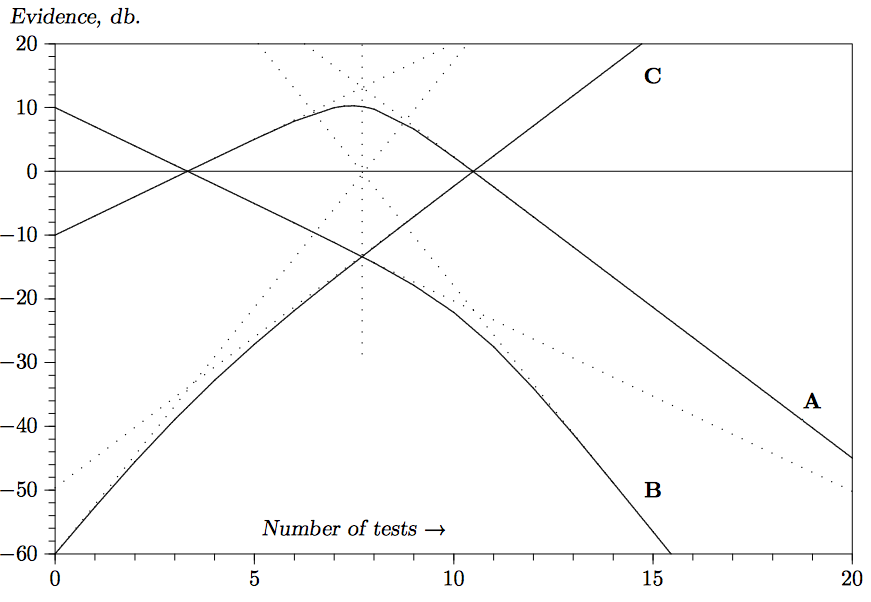
\includegraphics[width=0.5\textwidth]{mult_hyp_test.png}
                        \caption{Evidence for propositions $A$, $B$, and $C$ as a function of draws $m$. Note the peak in proposition $A$ at $\sim m = 7$.}
                    \end{figure}
                \item this is interesting, because initially $A$ and $C$ are so much more plausible than $C$ that we are functionally comparing $A$ and $C$ in binary
                \item once enough $e(C|DX) \approx e(B|DX)$, we are functionally testing $A$ against $C$, instead of against $B$
                \item all of the changes in slopes can be interpreted in this way, and this leads us to a general principle: 
                    \begin{displayquote}
                        As long as we have a discrete set of hypotheses, a change in plausibility for any one of them will be approximately the result of a test of this hypothesis against a single alternative, being one of the remaining hypotheses which is most plausible at that time.
                    \end{displayquote}
            \end{itemize}
    \end{itemize}

\subsection{Continuous probability distribution functions}
    \begin{itemize}
        \item we could continue the above example by adding in more and more `discrete' hypotheses.\ however a more interesting task would be to introduce a continuous range of hypotheses such that $H_f \equiv$ the machine putting out a fraction $f$ of fails
        \item instead of a discrete prior probability distribution, we would have a continous distribution in the interval $[0,1]$, and we could calculate posterior probabilities for various values of $f$
        \item suppose $f$ is any continuously variable parameter.\ the propositions 
            \begin{align*}
                F^{\prime} &\equiv (f \leq q) \\
                F^{\prime\prime} &\equiv (f > q)
            \end{align*}
        are discrete, mutually exclusive, and exhaustive
        \item with some prior information $Y$, the probability for $F^{\prime}$ will depend on $q$: $G(q) \equiv P(F^{\prime}|Y)$
        \item what is the probability  of finding $f$ in the interval $(a < f \leq b)$?
            \begin{itemize}
                \item Propositions:
                    \begin{equation*}
                        A \equiv (f \leq a) \hspace{0.5cm} B \equiv (f \leq b) \hspace{0.5cm} W \equiv (a < f \leq b)
                    \end{equation*}
                \item since $B = A + W$, and $A$ and $W$ are mutually exclusive, the sum rule is $P(B|Y) = P(A|Y) + P(W|Y)$
                \item and since $P(B|Y) = G(b)$ and $P(A|Y) = G(a)$, $P(W|Y) = P(a < f \leq b|Y) = G(b) - G(a)$
                \item if $G(q)$ is continuous and differentiable, we can also write $P(a < f \leq b|Y) = \int^b_{a} \mathrm{d}fg(f)$, where $g(f) = G^{\prime}(f) \geq 0$ is the derivative of $G$
                    \begin{itemize}
                        \item $G^{\prime}$ is the \textit{probability distribution function} (PDF) for $f$, given $Y$
                        \item should be noted that this is should not be described as a posterior probability \textbf{of} $f$, as that implies that $f$ is the thing being distributed.\ it is not, the \textit{probability} of $f$ is
                    \end{itemize}
            \end{itemize}
        \item it should be noticed that the same rules as we used in the treatment of discrete, finite sets of propositions were used here with a continuous, infinite set of propositions
            \begin{itemize}
                \item generally true if the continuous set of propositions is defined from a basis of finite sets of propositions
            \end{itemize}
    \end{itemize}

\subsection{Testing an infinite set of hypotheses}
    \begin{itemize}
        \item say we are testing an uncountable, infinite set of hypotheses.\ because log forms now become awkward (for some complicated reasons), we go back to using the original form for the probability of $P(A|DX)$ (the first equation in section 5.2)
        \item if $A$ is now the proposition that the fraction of fails is in teh range $(f, f + \mathrm{d}f)$, then the prior PDF is $P(A|X) = g(f|X)\mathrm{d}f$
        \item if $D$ is the data $N$ widgets were tested such that we found $n$ fails and $N-n$ good ones, the posterior PDF is 
            \begin{equation*}
                P(A|DX) = P(A|X) \frac{P(D|AX)}{P(D|X)} = g(f|DX)\mathrm{d}f
            \end{equation*}
        \item furthermore, the prior and posterior PDFs are related by
            \begin{equation*}
                g(f|DX) = g(f|X) \frac{P(D|AX)}{P(D|X)}
            \end{equation*}
        \item this problem is usually easier if we require that $P(0 \leq f \leq 1|DX) = \int^1_0 \mathrm{d}fg(f|DX) = 1$
        \item it should be clear that the evidence of the data is entirely within the $f$ dependence of $P(D|AX)$
        \item note that the proposition $A$ uses an interval $\mathrm{d}f$, not a point $f$ 
            \begin{itemize}
                \item if $f$ is the only variable, we can usually use the limit d$f \rightarrow 0$ and replace $P(D|AX)$ with $P(D|H_{f}X)$
                \item this only works reliably if $f$ is not dependent on any other variable, otherwise we don't know if d$f \rightarrow 0$ in the same way for all values of the other variable
                \item see the Borel-Kolmogorov paradox
            \end{itemize}
        \item if $f$ is the fraction of fails, then $(1-f)$ is the probability of getting a good one.\ the probabilities at different trials are logically independent given $f$, so we follow the binomial distribution and write
            \begin{equation}
                \label{binom_pdf}
                g(f|DX) = \frac{f^{n}{(1-f)}^{N-n}g(f|X)}{\int^1_{0}\mathrm{d}f{f^n(1-f)}^{N-n}g(f|X)}
            \end{equation}
            \begin{itemize}
                \item aside: this should absolutely evoke your first project derivation which has 
                    \begin{equation*}
                        P(\lambda, t) = \frac{\int \mathrm{d}x_0 \rho(x_0)h_{\mathrm{R}}(x_0) \delta[\lambda - \lambda(x_t)]}{\int \mathrm{d}x_0 \rho(x_0)h_{\mathrm{R}}(x_0)}
                    \end{equation*}
            \end{itemize}
        \item the entirety of the above section of multiple hypothesis testing can be dealt with using eq.~\ref{binom_pdf},\ using three delta functions for $g(f|X)$, $\delta(f-f_H)$, to denote the three hypotheses $A$, $B$, and $C$
        \item going back to the machine, what if the machine's starting information was simply that it was \textit{possible} for a machine to make a fail, and \textit{possible} for a machine to make a good one?
            \begin{itemize}
                \item we have no definite knowledge of a prior for $f$,\ and we haven't yet determined how to assign such priors
                \item best thing to do is definte a uniform prior PDF, $g(f|X) = 1$, where $0 \leq f \leq 1$
                \item eq.~\ref{binom_pdf} then reduces to the \textit{complete beta-function},
                    \begin{equation*}
                        g(f|DX) = \frac{(N+1)!}{n!(N-n)!} f^{n}{(1-f)}^{N-n}
                    \end{equation*}
                \item this has a single peak in the interval $(0 \leq f \leq 1)$, $f=\hat{f} \equiv \frac{n}{N}$, or the observed fraction of fails to good widgets
                \item the sharpness, however, is found by
                    \begin{equation*}
                        L(f) \equiv \log g(f|DX) = n\log(f) + (N-n)\log(1-f) + \mathrm{const}
                    \end{equation*}
                \item expanding $L(f)$ in a power series around $\hat{f}$,
                    \begin{equation*}
                        L(f) = L(\hat{f}) - \frac{{(f-\hat{f})}^2}{{2\sigma}^2}
                    \end{equation*}
                where 
                    \begin{equation*}
                        \sigma \equiv \frac{\hat{f}(1-\hat{f})}{N}
                    \end{equation*}
                \item and so the complete beta function in this approximation is 
                    \begin{equation}
                        \label{gauss}
                        g(f|DX) \approx K\exp\left[ - \frac{{(f-\hat{f})}^2}{{2\sigma}^2} \right]
                    \end{equation}
                which is the \textit{Gaussian distribution}
                \item so the most likely value of $f$ is the observed fraction $\hat{f}$, and the accuracy of this estimate is such that the interval $\hat{f} \pm \sigma$ is likely to contain the tru value
                \item $\sigma$ is the \textit{standard deviation} and ${\sigma}^2$ is the \textit{variance} of the PDF
                    \begin{itemize}
                        \item[] 50\% probability that the true value of $f$ is contained in the interval $\hat{f} \pm 0.68\sigma$
                        \item[] 90\% probability it is contained in $\hat{f} \pm 1.65\sigma$
                        \item[] 99\% probability it is contained in $\hat{f} \pm 2.57\sigma$
                    \end{itemize}
                \item as the number of tests $N$ increases, the intervals shrink proportional to $1/\sqrt{N}$
            \end{itemize}
    \end{itemize}

\subsection{Simple and compound hypotheses}
    \begin{itemize}
        \item so far the hypotheses we have considered refer to a single parameter, or value, $f = M/M$,\ and are sharply defined for this value $f$
        \item if we consider an abstract ``parameter space'' $\Omega$, consisting of all possible values of all possible parameters, these hypotheses are considered ``simple'' hypotheses as they refer to a single point within $\Omega$
        \item testing all simple hypotheses within $\Omega$ would be too much.\ could we test subsets, like ${\Omega}_1 \in \Omega$? can we proceed directly to this question instead of testing all possible simple hypotheses within ${\Omega}_1$?
            \begin{itemize}
                \item let's start from eq.~\ref{binom_pdf}.\ if we want to take some action with the machine, say readjust if $f > 0.1$, we can take some subset of $\Omega = [0,1]$, i.e.\ ${\Omega}_1$ comprising all $f$ in the interval $[0.1,1]$, and $H$ as the hypothesis that $f$ is in ${\Omega}_1$
                \item the actual value of $f$ is not needed anymore and is considered a \textit{nuisance parameter}, and we need to take action to remove it
                \item if there are no parameters other than $f$ and the intervals d$f$ are mutually exclusive, then $f$ is removed by integrating it out of eq~\ref{binom_pdf}:
                    \begin{equation*}
                        P(\Omega_1|DX) = \frac{\int_{\Omega_1}\mathrm{d}f f^n{(1-f)}^{N-n}g(f|X)}{\int_{\Omega}\mathrm{d}f f^n{(1-f)}^{N-n}g(f|X)} 
                    \end{equation*}
                and if we have a uniform prior PDF for $f$,
                    \begin{equation*}
                        P(a < f < b|DX) = \frac{(N+1)!}{n!(N-n)!}\int^b_{a}\mathrm{d}f f^n{(1-f)}^{N-n}
                    \end{equation*}
            \end{itemize}
        \item thus if we have any compound hypothesis to test, the proper procedure is to sum or integrate out the nuisance parameters the PDF contains, with respect to appropriate priors.
    \end{itemize}
\end{document}
